%% LyX 2.1.4 created this file.  For more info, see http://www.lyx.org/.
%% Do not edit unless you really know what you are doing.
\documentclass[twocolumn,english,journal]{IEEEtran}
\usepackage{newtxmath}
\usepackage[T1]{fontenc}
\usepackage[utf8]{inputenc}
\synctex=-1
\usepackage{babel}
\usepackage{float}
\usepackage{booktabs}
\usepackage{calc}
\usepackage[unicode=true,pdfusetitle,
 bookmarks=true,bookmarksnumbered=false,bookmarksopen=false,
 breaklinks=false,pdfborder={0 0 1},backref=false,colorlinks=false]
 {hyperref}

\makeatletter

%%%%%%%%%%%%%%%%%%%%%%%%%%%%%% LyX specific LaTeX commands.
%% Because html converters don't know tabularnewline
\providecommand{\tabularnewline}{\\}
\floatstyle{ruled}
\newfloat{algorithm}{tbp}{loa}
\providecommand{\algorithmname}{Algorithm}
\floatname{algorithm}{\protect\algorithmname}

%%%%%%%%%%%%%%%%%%%%%%%%%%%%%% Textclass specific LaTeX commands.
 % protect \markboth against an old bug reintroduced in babel >= 3.8g
 \let\oldforeign@language\foreign@language
 \DeclareRobustCommand{\foreign@language}[1]{%
   \lowercase{\oldforeign@language{#1}}}

%%%%%%%%%%%%%%%%%%%%%%%%%%%%%% User specified LaTeX commands.
\usepackage{graphicx}
\usepackage{pgfplots}
\usepgfplotslibrary{groupplots}
\pgfkeys{/pgf/number format/.cd, set thousands separator=\,}

\makeatother

\usepackage{listings}
\renewcommand{\lstlistingname}{Listing}

\begin{document}

\title{Title}


\author{Name and ID}


\markboth{Data Structures and Analysis of Algorithms -- Homework 1 -- My name}{}
\maketitle
\begin{abstract}
In this work\ldots{} For this,\ldots{} The results obtained\ldots{}
In conclusion,\ldots{} (everything in \emph{one} paragraph).
\end{abstract}


\section{Introduction}

\IEEEPARstart{In}{ this work}\ldots{} Lorem ipsum dolor sit amet,
consetetur sadipscing elitr, sed diam nonumy eirmod tempor invidunt
ut labore et dolore magna aliquyam erat, sed diam voluptua. At vero
eos et accusam et justo duo dolores et ea rebum. Stet clita kasd gubergren,
no sea takimata sanctus est Lorem ipsum dolor sit amet. Lorem ipsum
dolor sit amet, consetetur sadipscing elitr, sed diam nonumy eirmod
tempor invidunt ut labore et dolore magna aliquyam erat, sed diam
voluptua.

Lorem ipsum dolor sit amet, consetetur sadipscing elitr, sed diam
nonumy eirmod tempor invidunt ut labore et dolore magna aliquyam erat,
sed diam voluptua. At vero eos et accusam et justo duo dolores et
ea rebum. Stet clita kasd gubergren, no sea takimata sanctus est Lorem
ipsum dolor sit amet. Lorem ipsum dolor sit amet, consetetur sadipscing
elitr, sed diam nonumy eirmod tempor invidunt ut labore et dolore
magna aliquyam erat, sed diam voluptua.


\section{Methodology}

To answer this question\ldots{} Lorem ipsum dolor sit amet, consetetur
sadipscing elitr, sed diam nonumy eirmod tempor invidunt ut labore
et dolore magna aliquyam erat, sed diam voluptua. At vero eos et accusam
et justo duo dolores et ea rebum. Stet clita kasd gubergren, no sea
takimata sanctus est Lorem ipsum dolor sit amet. Lorem ipsum dolor
sit amet, consetetur sadipscing elitr, sed diam nonumy eirmod tempor
invidunt ut labore et dolore magna aliquyam erat, sed diam voluptua.

The code is shown in the appendix. It is based on the pseudocode in
the book of Cormen et al~\cite{Cormen:2009}. Lorem ipsum dolor sit
amet, consetetur sadipscing elitr, sed diam nonumy eirmod tempor invidunt
ut labore et dolore magna aliquyam erat, sed diam voluptua. At vero
eos et accusam et justo duo dolores et ea rebum. Stet clita kasd gubergren,
no sea takimata sanctus est Lorem ipsum dolor sit amet. Lorem ipsum
dolor sit amet, consetetur sadipscing elitr, sed diam nonumy eirmod
tempor invidunt ut labore et dolore magna aliquyam erat, sed diam
voluptua.

Lorem ipsum dolor sit amet, consetetur sadipscing elitr, sed diam
nonumy eirmod tempor invidunt ut labore et dolore magna aliquyam erat,
sed diam voluptua. At vero eos et accusam et justo duo dolores et
ea rebum. Stet clita kasd gubergren, no sea takimata sanctus est Lorem
ipsum dolor sit amet. Lorem ipsum dolor sit amet, consetetur sadipscing
elitr, sed diam nonumy eirmod tempor invidunt ut labore et dolore
magna aliquyam erat, sed diam voluptua.

Lorem ipsum dolor sit amet, consetetur sadipscing elitr, sed diam
nonumy eirmod tempor invidunt ut labore et dolore magna aliquyam erat,
sed diam voluptua. At vero eos et accusam et justo duo dolores et
ea rebum. Stet clita kasd gubergren, no sea takimata sanctus est Lorem
ipsum dolor sit amet. Lorem ipsum dolor sit amet, consetetur sadipscing
elitr, sed diam nonumy eirmod tempor invidunt ut labore et dolore
magna aliquyam erat, sed diam voluptua.


\section{Results}

The execution time of running teach of the algorithms several times
is shown in Table~\ref{tab:tiempos}.
\begin{table}
\caption{Execution time of sorting algorithms.\label{tab:tiempos}}


\centering{}%
\begin{tabular}{lrrrrrrr}
\toprule 
 &  & \multicolumn{6}{c}{Time (ms)}\tabularnewline
\cmidrule{3-8} 
 &  & \multicolumn{5}{c}{Execution} & \tabularnewline
\cmidrule{3-7} 
Algorithm & Size (k) & 1 & 2 & 3 & 4 & 5 & Mean\tabularnewline
\midrule 
Selection  & $10$ & $12.3$ & $12.3$ & $12.3$ & $12.3$ & $12.3$ & $12.3$\tabularnewline
 & $20$ & $12.3$ & $12.3$ & $12.3$ & $12.3$ & $12.3$ & $12.3$\tabularnewline
 & $30$ & $12.3$ & $12.3$ & $12.3$ & $12.3$ & $12.3$ & $12.3$\tabularnewline
 & $40$ & $12.3$ & $12.3$ & $12.3$ & $12.3$ & $12.3$ & $12.3$\tabularnewline
\midrule
Insertion  & $10$ & $12.3$ & $12.3$ & $12.3$ & $12.3$ & $12.3$ & $12.3$\tabularnewline
 & $20$ & $12.3$ & $12.3$ & $12.3$ & $12.3$ & $12.3$ & $12.3$\tabularnewline
 & $30$ & $12.3$ & $12.3$ & $12.3$ & $12.3$ & $12.3$ & $12.3$\tabularnewline
 & $40$ & $12.3$ & $12.3$ & $12.3$ & $12.3$ & $12.3$ & $12.3$\tabularnewline
\midrule
Merge  & $10$ & $12.3$ & $12.3$ & $12.3$ & $12.3$ & $12.3$ & $12.3$\tabularnewline
 & $20$ & $12.3$ & $12.3$ & $12.3$ & $12.3$ & $12.3$ & $12.3$\tabularnewline
 & $30$ & $12.3$ & $12.3$ & $12.3$ & $12.3$ & $12.3$ & $12.3$\tabularnewline
 & $40$ & $12.3$ & $12.3$ & $12.3$ & $12.3$ & $12.3$ & $12.3$\tabularnewline
\bottomrule
\end{tabular}
\end{table}
 Lorem ipsum dolor sit amet, consetetur sadipscing elitr, sed diam
nonumy eirmod tempor invidunt ut labore et dolore magna aliquyam erat,
sed diam voluptua. At vero eos et accusam et justo duo dolores et
ea rebum. Stet clita kasd gubergren, no sea takimata sanctus est Lorem
ipsum dolor sit amet. Lorem ipsum dolor sit amet, consetetur sadipscing
elitr, sed diam nonumy eirmod tempor invidunt ut labore et dolore
magna aliquyam erat, sed diam voluptua.

The mean execution times are plotted in Figure~\ref{fig:lin}.
\begin{figure*}
\begin{centering}
\begin{tikzpicture}
    \begin{axis}[name=plot1,width=0.9\columnwidth,xtick={10,20,...,40},ylabel=Time (ms),title=\textbf{Selection sort}]
        \addplot coordinates{(10,200) (20,600) (30,800) (40,1200)};
    \end{axis}
    \begin{axis}[name=plot2,at={($(plot1.east)+(0.15\textwidth,0)$)},anchor=west,width=0.9\columnwidth,xtick={10,20,...,40},title=\textbf{Insertion sort}]
        \addplot coordinates{(10,800) (20,1200) (30,400) (40,800)};
    \end{axis}
    \begin{axis}[name=plot3,at={($(plot1.south)-(0,1.5cm)$)},anchor=north,width=0.9\columnwidth,xtick={10,20,...,40},ylabel=Time (ms),title=\textbf{Merge sort}]
        \addplot coordinates{(10,600) (20,500) (30,100) (40,200)};
    \end{axis}
    \begin{axis}[name=plot4,at={($(plot2.south)-(0,1.5cm)$)},anchor=north,width=0.9\columnwidth,xtick={10,20,...,40},title=\textbf{Heapsort}]
        \addplot coordinates{(10,600) (20,100) (30,500) (40,100)};
    \end{axis}
    \begin{axis}[name=plot5,at={($(plot3.south)-(0,1.5cm)$)},anchor=north,width=0.9\columnwidth,ylabel=Time (ms),xlabel=Array size (k),title=\textbf{Quicksort}]
        \addplot coordinates{(10,300) (20,100) (30,200) (40,500)};
    \end{axis}
% Comente las líneas siguientes con '%' si no implementó ordenamiento por Radix sort
  \begin{axis}[name=plot6,at={($(plot4.south)-(0,1.5cm)$)},anchor=north,width=0.9\columnwidth,xlabel=Array size (k),title=\textbf{Radix sort}]
        \addplot coordinates{(10,600) (20,200) (30,400) (40,500)};
    \end{axis}
\end{tikzpicture}
\par\end{centering}

\caption{Average execution time of sorting algorithms. \label{fig:lin}}
\end{figure*}
 The shape of the curves was not as expected because we made up the
numbers. Lorem ipsum dolor sit amet, consetetur sadipscing elitr,
sed diam nonumy eirmod tempor invidunt ut labore et dolore magna aliquyam
erat, sed diam voluptua. At vero eos et accusam et justo duo dolores
et ea rebum. Stet clita kasd gubergren, no sea takimata sanctus est
Lorem ipsum dolor sit amet. Lorem ipsum dolor sit amet, consetetur
sadipscing elitr, sed diam nonumy eirmod tempor invidunt ut labore
et dolore magna aliquyam erat, sed diam voluptua.

For comparison purposes, the curves are shown together in the same
graph in Figure~\ref{fig:log}.
\begin{figure*}
\begin{centering}
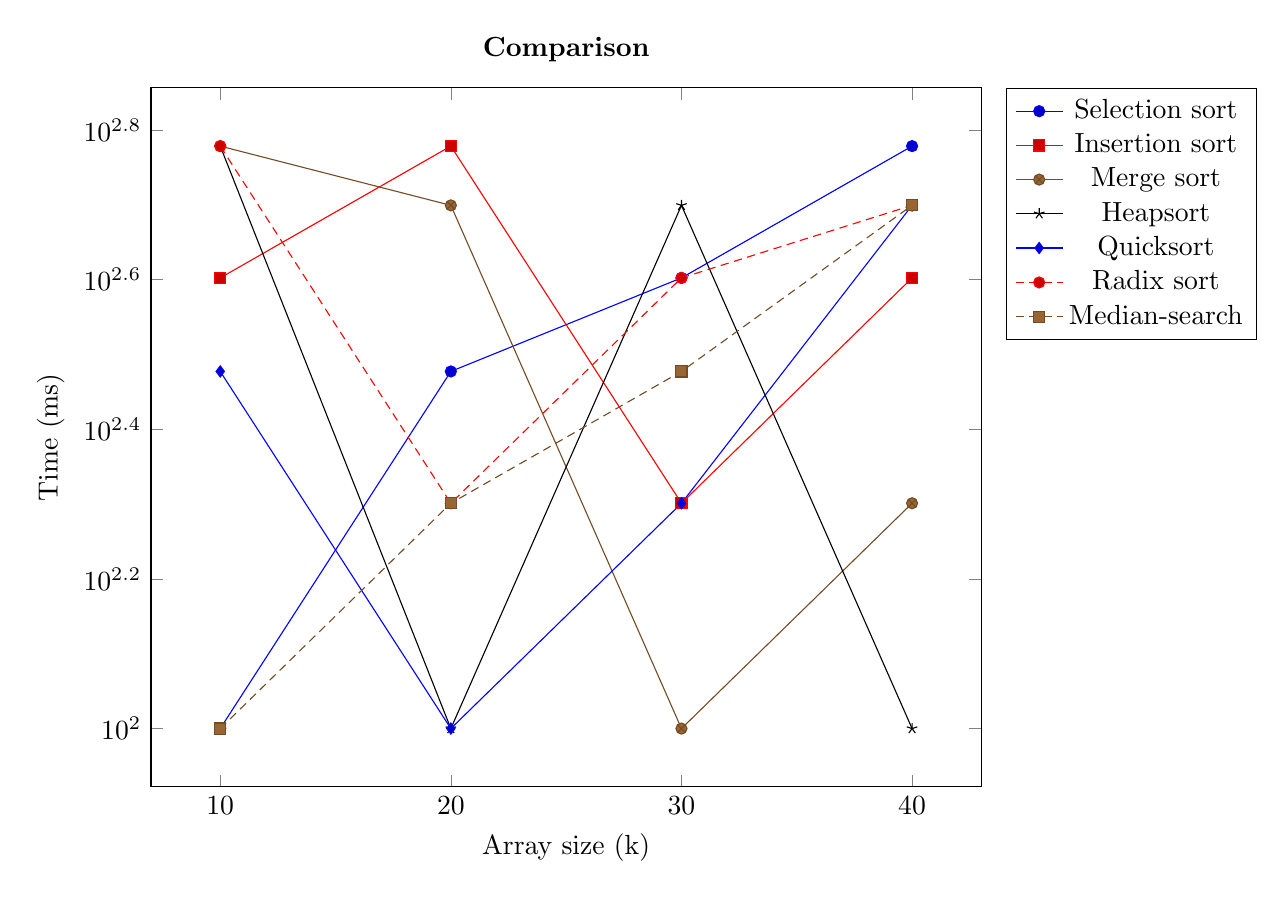
\begin{tikzpicture} 
    \begin{semilogyaxis}[
         width=\columnwidth,
         xtick={10,20,...,40},
         xlabel=Array size (k),
         ylabel=Time (ms),
         legend pos=outer north east,
         title=\textbf{Comparison}]
    \addplot coordinates{(10,100) (20,300) (30,400) (40,600)};
    \addplot coordinates{(10,400) (20,600) (30,200) (40,400)};
    \addplot coordinates{(10,600) (20,500) (30,100) (40,200)};
    \addplot coordinates{(10,600) (20,100) (30,500) (40,100)};
    \addplot coordinates{(10,300) (20,100) (30,200) (40,500)};
    \addplot coordinates{(10,600) (20,200) (30,400) (40,500)};
    \addplot coordinates{(10,100) (20,200) (30,300) (40,500)};
    \legend{Selection sort,Insertion sort,Merge sort,Heapsort,Quicksort,Radix sort,Median-search}
    \end{semilogyaxis}
\end{tikzpicture}
\par\end{centering}

\caption{Comparing mean running times of sorting algorithms.\label{fig:log}}
\end{figure*}
 No comments\ldots{} Lorem ipsum dolor sit amet, consetetur sadipscing
elitr, sed diam nonumy eirmod tempor invidunt ut labore et dolore
magna aliquyam erat, sed diam voluptua. At vero eos et accusam et
justo duo dolores et ea rebum. Stet clita kasd gubergren, no sea takimata
sanctus est Lorem ipsum dolor sit amet. Lorem ipsum dolor sit amet,
consetetur sadipscing elitr, sed diam nonumy eirmod tempor invidunt
ut labore et dolore magna aliquyam erat, sed diam voluptua.


\section{Conclusions}

From the results we can conclude that\ldots{} Lorem ipsum dolor sit
amet, consetetur sadipscing elitr, sed diam nonumy eirmod tempor invidunt
ut labore et dolore magna aliquyam erat, sed diam voluptua. At vero
eos et accusam et justo duo dolores et ea rebum. Stet clita kasd gubergren,
no sea takimata sanctus est Lorem ipsum dolor sit amet. Lorem ipsum
dolor sit amet, consetetur sadipscing elitr, sed diam nonumy eirmod
tempor invidunt ut labore et dolore magna aliquyam erat, sed diam
voluptua.

Lorem ipsum dolor sit amet, consetetur sadipscing elitr, sed diam
nonumy eirmod tempor invidunt ut labore et dolore magna aliquyam erat,
sed diam voluptua. At vero eos et accusam et justo duo dolores et
ea rebum. Stet clita kasd gubergren, no sea takimata sanctus est Lorem
ipsum dolor sit amet. Lorem ipsum dolor sit amet, consetetur sadipscing
elitr, sed diam nonumy eirmod tempor invidunt ut labore et dolore
magna aliquyam erat, sed diam voluptua.


\appendices{}


\section{Code}

Algorithms \ref{alg:pura-vida} and \ref{alg:hello-world} show the
code used in this work.

\begin{algorithm}
\caption{Algorithm that displays Tico's most popular expression.\label{alg:pura-vida}}


\begin{lstlisting}[language={[ANSI]C++}]
int main() {
	cout << 'Pura vida!\n';
	return 0; 
}
\end{lstlisting}
\end{algorithm}
\begin{algorithm*}
\caption{First program of any Computer Science student. If the code does not
fit in one column, use the \textquotedblleft span columns\textquotedblright{}
option in the settings of the float (just like this floating algorithm).
In \protect\LaTeX{} use the \emph{starred} version of algorithm (i.e., \texttt{\textbackslash{}begin\{algorithm{*}\}}
and \texttt{\textbackslash{}end\{algorithm{*}\}})\label{alg:hello-world}}


\lstinputlisting[language={C++}]{Hello_world.cpp}
\end{algorithm*}


\bibliographystyle{IEEEtran}
\bibliography{Referencias}

\begin{IEEEbiography}[{\fbox{\begin{minipage}[t][1.25in]{1in}%
Replace this box by an image with a width of 1\,in and a height of
1.25\,in!%
\end{minipage}}}]{Your Name}
 All about you and the what your interests are.\end{IEEEbiography}


\end{document}
